
%% bare_conf.tex
%% V1.3
%% 2007/01/11
%% by Michael Shell
%% See:
%% http://www.michaelshell.org/
%% for current contact information.
%%
%% This is a skeleton file demonstrating the use of IEEEtran.cls
%% (requires IEEEtran.cls version 1.7 or later) with an IEEE conference paper.
%%
%% Support sites:
%% http://www.michaelshell.org/tex/ieeetran/
%% http://www.ctan.org/tex-archive/macros/latex/contrib/IEEEtran/
%% and
%% http://www.ieee.org/

%%*************************************************************************
%% Legal Notice:
%% This code is offered as-is without any warranty either expressed or
%% implied; without even the implied warranty of MERCHANTABILITY or
%% FITNESS FOR A PARTICULAR PURPOSE! 
%% User assumes all risk.
%% In no event shall IEEE or any contributor to this code be liable for
%% any damages or losses, including, but not limited to, incidental,
%% consequential, or any other damages, resulting from the use or misuse
%% of any information contained here.
%%
%% All comments are the opinions of their respective authors and are not
%% necessarily endorsed by the IEEE.
%%
%% This work is distributed under the LaTeX Project Public License (LPPL)
%% ( http://www.latex-project.org/ ) version 1.3, and may be freely used,
%% distributed and modified. A copy of the LPPL, version 1.3, is included
%% in the base LaTeX documentation of all distributions of LaTeX released
%% 2003/12/01 or later.
%% Retain all contribution notices and credits.
%% ** Modified files should be clearly indicated as such, including  **
%% ** renaming them and changing author support contact information. **
%%
%% File list of work: IEEEtran.cls, IEEEtran_HOWTO.pdf, bare_adv.tex,
%%                    bare_conf.tex, bare_jrnl.tex, bare_jrnl_compsoc.tex
%%*************************************************************************

% *** Authors should verify (and, if needed, correct) their LaTeX system  ***
% *** with the testflow diagnostic prior to trusting their LaTeX platform ***
% *** with production work. IEEE's font choices can trigger bugs that do  ***
% *** not appear when using other class files.                            ***
% The testflow support page is at:
% http://www.michaelshell.org/tex/testflow/



% Note that the a4paper option is mainly intended so that authors in
% countries using A4 can easily print to A4 and see how their papers will
% look in print - the typesetting of the document will not typically be
% affected with changes in paper size (but the bottom and side margins will).
% Use the testflow package mentioned above to verify correct handling of
% both paper sizes by the user's LaTeX system.
%
% Also note that the "draftcls" or "draftclsnofoot", not "draft", option
% should be used if it is desired that the figures are to be displayed in
% draft mode.
%
\documentclass[conference]{IEEEtran}
\usepackage{blindtext, graphicx}
% Add the compsoc option for Computer Society conferences.
%
% If IEEEtran.cls has not been installed into the LaTeX system files,
% manually specify the path to it like:
% \documentclass[conference]{../sty/IEEEtran}





% Some very useful LaTeX packages include:
% (uncomment the ones you want to load)


% *** MISC UTILITY PACKAGES ***
%
%\usepackage{ifpdf}
% Heiko Oberdiek's ifpdf.sty is very useful if you need conditional
% compilation based on whether the output is pdf or dvi.
% usage:
% \ifpdf
%   % pdf code
% \else
%   % dvi code
% \fi
% The latest version of ifpdf.sty can be obtained from:
% http://www.ctan.org/tex-archive/macros/latex/contrib/oberdiek/
% Also, note that IEEEtran.cls V1.7 and later provides a builtin
% \ifCLASSINFOpdf conditional that works the same way.
% When switching from latex to pdflatex and vice-versa, the compiler may
% have to be run twice to clear warning/error messages.






% *** CITATION PACKAGES ***
%
%\usepackage{cite}
% cite.sty was written by Donald Arseneau
% V1.6 and later of IEEEtran pre-defines the format of the cite.sty package
% \cite{} output to follow that of IEEE. Loading the cite package will
% result in citation numbers being automatically sorted and properly
% "compressed/ranged". e.g., [1], [9], [2], [7], [5], [6] without using
% cite.sty will become [1], [2], [5]--[7], [9] using cite.sty. cite.sty's
% \cite will automatically add leading space, if needed. Use cite.sty's
% noadjust option (cite.sty V3.8 and later) if you want to turn this off.
% cite.sty is already installed on most LaTeX systems. Be sure and use
% version 4.0 (2003-05-27) and later if using hyperref.sty. cite.sty does
% not currently provide for hyperlinked citations.
% The latest version can be obtained at:
% http://www.ctan.org/tex-archive/macros/latex/contrib/cite/
% The documentation is contained in the cite.sty file itself.






% *** GRAPHICS RELATED PACKAGES ***
%
\ifCLASSINFOpdf
  % \usepackage[pdftex]{graphicx}
  % declare the path(s) where your graphic files are
  % \graphicspath{{../pdf/}{../jpeg/}}
  % and their extensions so you won't have to specify these with
  % every instance of \includegraphics
  % \DeclareGraphicsExtensions{.pdf,.jpeg,.png}
\else
  % or other class option (dvipsone, dvipdf, if not using dvips). graphicx
  % will default to the driver specified in the system graphics.cfg if no
  % driver is specified.
  % \usepackage[dvips]{graphicx}
  % declare the path(s) where your graphic files are
  % \graphicspath{{../eps/}}
  % and their extensions so you won't have to specify these with
  % every instance of \includegraphics
  % \DeclareGraphicsExtensions{.eps}
\fi
% graphicx was written by David Carlisle and Sebastian Rahtz. It is
% required if you want graphics, photos, etc. graphicx.sty is already
% installed on most LaTeX systems. The latest version and documentation can
% be obtained at: 
% http://www.ctan.org/tex-archive/macros/latex/required/graphics/
% Another good source of documentation is "Using Imported Graphics in
% LaTeX2e" by Keith Reckdahl which can be found as epslatex.ps or
% epslatex.pdf at: http://www.ctan.org/tex-archive/info/
%
% latex, and pdflatex in dvi mode, support graphics in encapsulated
% postscript (.eps) format. pdflatex in pdf mode supports graphics
% in .pdf, .jpeg, .png and .mps (metapost) formats. Users should ensure
% that all non-photo figures use a vector format (.eps, .pdf, .mps) and
% not a bitmapped formats (.jpeg, .png). IEEE frowns on bitmapped formats
% which can result in "jaggedy"/blurry rendering of lines and letters as
% well as large increases in file sizes.
%
% You can find documentation about the pdfTeX application at:
% http://www.tug.org/applications/pdftex





% *** MATH PACKAGES ***
%
%\usepackage[cmex10]{amsmath}
% A popular package from the American Mathematical Society that provides
% many useful and powerful commands for dealing with mathematics. If using
% it, be sure to load this package with the cmex10 option to ensure that
% only type 1 fonts will utilized at all point sizes. Without this option,
% it is possible that some math symbols, particularly those within
% footnotes, will be rendered in bitmap form which will result in a
% document that can not be IEEE Xplore compliant!
%
% Also, note that the amsmath package sets \interdisplaylinepenalty to 10000
% thus preventing page breaks from occurring within multiline equations. Use:
%\interdisplaylinepenalty=2500
% after loading amsmath to restore such page breaks as IEEEtran.cls normally
% does. amsmath.sty is already installed on most LaTeX systems. The latest
% version and documentation can be obtained at:
% http://www.ctan.org/tex-archive/macros/latex/required/amslatex/math/





% *** SPECIALIZED LIST PACKAGES ***
%
%\usepackage{algorithmic}
% algorithmic.sty was written by Peter Williams and Rogerio Brito.
% This package provides an algorithmic environment fo describing algorithms.
% You can use the algorithmic environment in-text or within a figure
% environment to provide for a floating algorithm. Do NOT use the algorithm
% floating environment provided by algorithm.sty (by the same authors) or
% algorithm2e.sty (by Christophe Fiorio) as IEEE does not use dedicated
% algorithm float types and packages that provide these will not provide
% correct IEEE style captions. The latest version and documentation of
% algorithmic.sty can be obtained at:
% http://www.ctan.org/tex-archive/macros/latex/contrib/algorithms/
% There is also a support site at:
% http://algorithms.berlios.de/index.html
% Also of interest may be the (relatively newer and more customizable)
% algorithmicx.sty package by Szasz Janos:
% http://www.ctan.org/tex-archive/macros/latex/contrib/algorithmicx/




% *** ALIGNMENT PACKAGES ***
%
%\usepackage{array}
% Frank Mittelbach's and David Carlisle's array.sty patches and improves
% the standard LaTeX2e array and tabular environments to provide better
% appearance and additional user controls. As the default LaTeX2e table
% generation code is lacking to the point of almost being broken with
% respect to the quality of the end results, all users are strongly
% advised to use an enhanced (at the very least that provided by array.sty)
% set of table tools. array.sty is already installed on most systems. The
% latest version and documentation can be obtained at:
% http://www.ctan.org/tex-archive/macros/latex/required/tools/


%\usepackage{mdwmath}
%\usepackage{mdwtab}
% Also highly recommended is Mark Wooding's extremely powerful MDW tools,
% especially mdwmath.sty and mdwtab.sty which are used to format equations
% and tables, respectively. The MDWtools set is already installed on most
% LaTeX systems. The lastest version and documentation is available at:
% http://www.ctan.org/tex-archive/macros/latex/contrib/mdwtools/


% IEEEtran contains the IEEEeqnarray family of commands that can be used to
% generate multiline equations as well as matrices, tables, etc., of high
% quality.


%\usepackage{eqparbox}
% Also of notable interest is Scott Pakin's eqparbox package for creating
% (automatically sized) equal width boxes - aka "natural width parboxes".
% Available at:
% http://www.ctan.org/tex-archive/macros/latex/contrib/eqparbox/





% *** SUBFIGURE PACKAGES ***
%\usepackage[tight,footnotesize]{subfigure}
% subfigure.sty was written by Steven Douglas Cochran. This package makes it
% easy to put subfigures in your figures. e.g., "Figure 1a and 1b". For IEEE
% work, it is a good idea to load it with the tight package option to reduce
% the amount of white space around the subfigures. subfigure.sty is already
% installed on most LaTeX systems. The latest version and documentation can
% be obtained at:
% http://www.ctan.org/tex-archive/obsolete/macros/latex/contrib/subfigure/
% subfigure.sty has been superceeded by subfig.sty.



%\usepackage[caption=false]{caption}
%\usepackage[font=footnotesize]{subfig}
% subfig.sty, also written by Steven Douglas Cochran, is the modern
% replacement for subfigure.sty. However, subfig.sty requires and
% automatically loads Axel Sommerfeldt's caption.sty which will override
% IEEEtran.cls handling of captions and this will result in nonIEEE style
% figure/table captions. To prevent this problem, be sure and preload
% caption.sty with its "caption=false" package option. This is will preserve
% IEEEtran.cls handing of captions. Version 1.3 (2005/06/28) and later 
% (recommended due to many improvements over 1.2) of subfig.sty supports
% the caption=false option directly:
%\usepackage[caption=false,font=footnotesize]{subfig}
%
% The latest version and documentation can be obtained at:
% http://www.ctan.org/tex-archive/macros/latex/contrib/subfig/
% The latest version and documentation of caption.sty can be obtained at:
% http://www.ctan.org/tex-archive/macros/latex/contrib/caption/




% *** FLOAT PACKAGES ***
%
%\usepackage{fixltx2e}
% fixltx2e, the successor to the earlier fix2col.sty, was written by
% Frank Mittelbach and David Carlisle. This package corrects a few problems
% in the LaTeX2e kernel, the most notable of which is that in current
% LaTeX2e releases, the ordering of single and double column floats is not
% guaranteed to be preserved. Thus, an unpatched LaTeX2e can allow a
% single column figure to be placed prior to an earlier double column
% figure. The latest version and documentation can be found at:
% http://www.ctan.org/tex-archive/macros/latex/base/



%\usepackage{stfloats}
% stfloats.sty was written by Sigitas Tolusis. This package gives LaTeX2e
% the ability to do double column floats at the bottom of the page as well
% as the top. (e.g., "\begin{figure*}[!b]" is not normally possible in
% LaTeX2e). It also provides a command:
%\fnbelowfloat
% to enable the placement of footnotes below bottom floats (the standard
% LaTeX2e kernel puts them above bottom floats). This is an invasive package
% which rewrites many portions of the LaTeX2e float routines. It may not work
% with other packages that modify the LaTeX2e float routines. The latest
% version and documentation can be obtained at:
% http://www.ctan.org/tex-archive/macros/latex/contrib/sttools/
% Documentation is contained in the stfloats.sty comments as well as in the
% presfull.pdf file. Do not use the stfloats baselinefloat ability as IEEE
% does not allow \baselineskip to stretch. Authors submitting work to the
% IEEE should note that IEEE rarely uses double column equations and
% that authors should try to avoid such use. Do not be tempted to use the
% cuted.sty or midfloat.sty packages (also by Sigitas Tolusis) as IEEE does
% not format its papers in such ways.





% *** PDF, URL AND HYPERLINK PACKAGES ***
%
%\usepackage{url}
% url.sty was written by Donald Arseneau. It provides better support for
% handling and breaking URLs. url.sty is already installed on most LaTeX
% systems. The latest version can be obtained at:
% http://www.ctan.org/tex-archive/macros/latex/contrib/misc/
% Read the url.sty source comments for usage information. Basically,
% \url{my_url_here}.





% *** Do not adjust lengths that control margins, column widths, etc. ***
% *** Do not use packages that alter fonts (such as pslatex).         ***
% There should be no need to do such things with IEEEtran.cls V1.6 and later.
% (Unless specifically asked to do so by the journal or conference you plan
% to submit to, of course. )


% correct bad hyphenation here
\hyphenation{op-tical net-works semi-conduc-tor}

\usepackage{hyperref}

\usepackage{amsmath}
\DeclareMathOperator*{\argmin}{arg\,min}

\begin{document}
%
% paper title
% can use linebreaks \\ within to get better formatting as desired
\title{Behavioral authentication by cursor tracking}


% author names and affiliations
% use a multiple column layout for up to three different
% affiliations
\author{\IEEEauthorblockN{Felix Neutatz}
\IEEEauthorblockA{School of Electronic Information and\\Electrical Engineering\\
Shanghai Jiao Tong University\\
Email: neutatz@gmail.com}}

% conference papers do not typically use \thanks and this command
% is locked out in conference mode. If really needed, such as for
% the acknowledgment of grants, issue a \IEEEoverridecommandlockouts
% after \documentclass

% for over three affiliations, or if they all won't fit within the width
% of the page, use this alternative format:
% 
%\author{\IEEEauthorblockN{Michael Shell\IEEEauthorrefmark{1},
%Homer Simpson\IEEEauthorrefmark{2},
%James Kirk\IEEEauthorrefmark{3}, 
%Montgomery Scott\IEEEauthorrefmark{3} and
%Eldon Tyrell\IEEEauthorrefmark{4}}
%\IEEEauthorblockA{\IEEEauthorrefmark{1}School of Electrical and Computer Engineering\\
%Georgia Institute of Technology,
%Atlanta, Georgia 30332--0250\\ Email: see http://www.michaelshell.org/contact.html}
%\IEEEauthorblockA{\IEEEauthorrefmark{2}Twentieth Century Fox, Springfield, USA\\
%Email: homer@thesimpsons.com}
%\IEEEauthorblockA{\IEEEauthorrefmark{3}Starfleet Academy, San Francisco, California 96678-2391\\
%Telephone: (800) 555--1212, Fax: (888) 555--1212}
%\IEEEauthorblockA{\IEEEauthorrefmark{4}Tyrell Inc., 123 Replicant Street, Los Angeles, California 90210--4321}}




% use for special paper notices
%\IEEEspecialpapernotice{(Invited Paper)}




% make the title area
\maketitle


\begin{abstract}
We present an approach to a mostly unsupervised user authentication and identification based on
mouse dynamics. Our hypothesis is that one can successfully identify a user on the basis of cursor movements.
Our system identifies a user as unauthorized if the behavior within a 10 seconds period deviates sufficiently from the learned behavior of an authorized user.
Our results for four users show that we can identify these as unauthorized based on their cursor dynamics with
a false positive rate of 0\% and a false negative rate of 20\% on the authorized user data. Nevertheless, we have to research more thoroughly and use more data to validate our results. We point out that analysing cursor dynamics alone is not yet sufficient for a practical user authentication system.
\end{abstract}
% IEEEtran.cls defaults to using nonbold math in the Abstract.
% This preserves the distinction between vectors and scalars. However,
% if the journal you are submitting to favors bold math in the abstract,
% then you can use LaTeX's standard command \boldmath at the very start
% of the abstract to achieve this. Many IEEE journals frown on math
% in the abstract anyway.

% Note that keywords are not normally used for peerreview papers.
\begin{IEEEkeywords}
user verification, mouse dynamics, anomaly detection.
\end{IEEEkeywords}






% For peer review papers, you can put extra information on the cover
% page as needed:
% \ifCLASSOPTIONpeerreview
% \begin{center} \bfseries EDICS Category: 3-BBND \end{center}
% \fi
%
% For peerreview papers, this IEEEtran command inserts a page break and
% creates the second title. It will be ignored for other modes.
\IEEEpeerreviewmaketitle



\section{Introduction}

Authentication plays a major role in securing a system today. There are three main ways to tackle the problem of authentication. The user can be identified by knowledge (e.g. passwords, PIN), by possession (e.g. RFID \cite{feldhofer2004strong}, smart cards \cite{deo1998authentication}) or by the user himself/herself (e.g. voice \cite{kennedy2000radio}, face \cite{mallauran2005online}, iris \cite{chong2005iris} detection and fingerprint \cite{gupta2005efficient} recognition). \cite{pusara2004user} The first two ways have their weaknesses. The concept of possession is not bulletproof. The tokens can be stolen and/or copied.
With increasing computation capabilities, passwords can be cracked using brute force attacks in shorter time periods. Especially when quantum computing is understood, it will be trivial to calculate almost any password. \cite{steane1998quantum} Another problem of knowledge is the human factor. Humans forget. So you have to install processes for the case of resetting a password. These can be exploited using social engineering as a hacker used against Central Intelligence Agency (CIA) Director John Brennan. \cite{wiredSocialEng} Biometric authentication is a bit more secure, but these methods can also be cracked by e.g. taking a photo of the finger, iris, ...
An interesting step ahead is research on gait authentication. \cite{gafurov2006biometric} So instead of using the properties of a person, the actions and behavior is used to identify a person. The behavior of a person is hard to fake, maybe not at all.
So it is interesting to apply this idea on personal computer authentication.

There are many ways to track the behavior of computer users, but in this paper we want to focus on the cursor position over time. This can be seen as a first step to research whether our approach works in general. Mouse tracking on its own is not enough for computer authentication since the user can navigate by keyboard only. So this model will be extended to keyboard input in the future.

Monitoring the behavior of user has one main advantage over the common authentication: The user doesn't need to log off the system. So there is no way that you forget to log off. This is one of the key advantages of behavioral authentication because it is less susceptible to insider attacks. According to the US State of Cybercrime Survey \cite{us2014us}, "Almost one-third (32\%) say insider crimes are more costly or damaging than incidents perpetrated by outsiders.". So this can be critical.

The quality of an authentication method is based on its accuracy, how fast it can recognize the user and how difficult it is to circumvent it. It is extremely hard to simulate a person's behavior, so this criterion is already met for this method. So in this paper we focus on achieving also the other two.

The remainder of the paper is structured as follows: Section \ref{sec:relwork} discusses the related work. Section \ref{sec:approach} introduces user
authentication via mouse dynamics and describes a mostly unsupervised learning method for modeling user behavior. Section \ref{sec:conclusion} summarizes and discusses future research directions.

%describe data

\section{Related work}
\label{sec:relwork}

One of the first papers on the idea of authentication by behavioral patterns was published by Denning in 1985 \cite{denning1985requirements}. Moreover there are already a lot publications about authentication by analysing mouse dynamics. Pusara et al. show that you can differentiate users by their cursor movement with a very low error rate \cite{pusara2004user}. Zheng et al. extended their work by developing an angle-based feature set which could reduce the recording time to a time span of 20 mouse clicks. \cite{zheng2011efficient} Gamboa et al. came up with a 63-dimensional feature vector and showed the error for a different number of strokes (segment between two mouse clicks). \cite{gamboa2003identity} However, all these methods are purely supervised learning methods and based on training on data of several users.

In this paper we present a mostly unsupervised user authentication system that builds a model of a user’s behavior from his/her mouse dynamics without using data from other users. Therefore this approach introduces less privacy issues. Moreover we don't use mouse events in the data. This causes a disadvantage in comparison to the papers described before, because we have less information. Therefore we can exploit less entropy. But this will change in future work.

\section{User authentication via mouse dynamics}
\label{sec:approach}

As introduced in \cite{pusara2004user}, we use an unsupervised method to identify users. We model the behavior of the authorized user and apply this model on the mouse movements of any user. The idea is that if this model reproduces the given data very good, the probability that the data originated from the authorized user is very high. This corresponds to the problem of an anomaly detection task. The norm is the user's model and the anomaly is an unauthorized user.

\subsection{Data set}

For the authorized user we recorded the mouse position for 1h. To test the model for unauthorized users we recorded 4 different persons for 10 seconds. This is a very marginal data set. Extending this data set or applying the method on another data set will be also part of future work. 
The recoding keeps track of the x- and y-coordinate of the cursor every 30 milliseconds. In comparison to Pusara \cite{pusara2004user} we can leverage about 3 times more data, because our monitoring frequency is higher. Our model is based on equidistant data points in time. Therefore we focus on this to ensure this constraint. This requires a lot of unnecessary computation. Therefore another task for future work would be to find a model which can incorporate non-equidistant data points.
The coordinates are normalized by screen size. 

\subsection{Anomaly detection}

To model the user behavior of an authorized user we use linear regression. The idea is to fit a model which is capable of reconstructing the training data. For example that means predicting the cursor position at time t given that you know at which position the mouse was 1, ..., k time steps ago. In this way we can calculate the
coefficients accordingly and find the best model which excels in predicting and reconstructing sequential data. This approach was introduced by Dunning \cite{dunning2014practical}. This is an unsupervised problem because we can only train on records of class "authorized user". So there is no value in the label of the observations which forces us to work without labels. Reformulating this problem to be a sequence reconstruction problem makes it supervised again.

To train a model we use linear regression. In the general case the model of linear regression is described in the following way:

\begin{equation}
y = a^{T} x
\end{equation}

In our case linear regression solves the following problem: 

\begin{equation}
y_{t} = a_{0} + a_{1} * x_{t - 1 * 0.03s} + ... + a_{k} * x_{t - k * 0.03s}
\end{equation}

such that the sum of squared residuals is minimized:

\begin{equation}
\label{eq:problem}
\argmin_{a} \sum (y - a^T*x)^2
\end{equation}

In this case linear regression solves a constrained optimization problem. The target values are within the interval [0,1] because otherwise this would mean it would be possible for the cursor to leave the screen. To solve this problem we set the predicted value to 0 if it is smaller than 0 and 1 if it is bigger than 1. In future work we will elaborate what the best optimization strategy is to solve such a problem.


\subsubsection{Training}

For the training of the linear regression model for the authorized user we first analyse a recording of one hour. 40 \% of the data is used as the validation set. To understand how much improvement we gain by training on more data we run an experiment using k = 100 (figure \ref{fig_trainingsize}) which shows that the accuracy is starting to converge using the whole validation set (36 min). This means that it suffices to use 1h as training data.

\begin{figure}[!t]
\centering
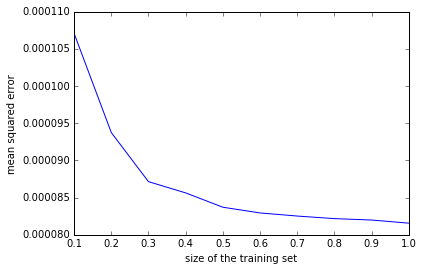
\includegraphics[width=2.5in]{img/error_trainingsize.png}
\caption{Error by training set size}
\label{fig_trainingsize}
\end{figure}

\subsubsection{Feature selection}

The challenge of feature selection in this case is the trade-off between the information gain and how fast we can classify a sample. This means if we could decide that the model should predict the next mouse position by only knowing the previous cursor position. So theoretically we would only need 30 ms to be able to classify whether it is an authorized user. But the downside is that the model is not very good, because it is hard to learn only by one previous step. One the other hand we could decide to give the model the last 1000 steps. The model would have a high accuracy but that would also mean that we have to wait for 30 seconds until we are able to classify. So the question to answer is how many steps do we let the model look back into the past. We run an experiment to find a good middle way. Figure \ref{fig_features} shows the mean squared error on a test set using k features or looking k times steps back, respectively. It turns out that the error flattens more and more. It only decreases minimally after k=100. So we decide to use 100 time steps in our experiments.

\begin{figure}[!t]
\centering
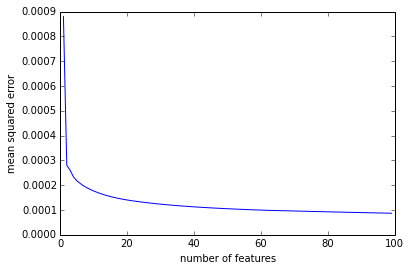
\includegraphics[width=2.5in]{img/error_features.png}
\caption{Error by number of features}
\label{fig_features}
\end{figure}

\subsubsection{Model evaluation}
As test set we use a two hour recording of the authorized user. Table \ref{table_model_quality} shows that training and validation error are almost the same which is a clear sign that the model doesn't suffer from overfitting. The mean squared test error is twice as high as the validation error, but is still very low. These results show that the model is good in predicting cursor dynamics.

\begin{table}[!t]
\renewcommand{\arraystretch}{1.3}
% \extrarowheight as needed to properly center the text within the cells
\caption{Authorized user behavior model - accuracy (Mean squared error)}
\label{table_model_quality}
\centering
\begin{tabular}{|c||c|c|c|}
\hline
Metric & Training error & Validation error & Test Error\\
 & (36 min) & (24 min) & (120 min)\\
\hline
MSE & 0.00007866 & 0.00007826 & 0.00016176\\
\hline
Distance normed MSE & 0.0221 & 0.0183 & 0.0299\\
\hline
Smoothed MSE & 3.23e-07 & 3.42e-07 & 4.02e-07\\
\hline
Distance smoothed MSE & 0.179 & 0.168 & 0.160\\
\hline
\end{tabular}
\end{table}


\subsubsection{Error metrics}
We need a good error metric to be able to compare the error of an authorized user and a non-authorized user. First, we try mean squared error (showed in equation \ref{eq:mse}). The problem of the mean squared error is that it doesn't take into account the amount of "no movement". This means if there is no movement at all it is very easy to classify and therefore the mean squared error will be small. So the amount of "no movement" matters. To avoid this effect we delete all samples which have a past of no movement (all previous k time steps doesn't change in position). We apply this procedure also on the training data which increases the accuracy and speeds up training.

\begin{equation}
\label{eq:mse}
\frac{1}{n} \sum_{i=1}^{n}  (y_{i} - a^T*x_{i})^2
\end{equation}

But there is still an issue with that metric. It is harder for the model to classify when you move the mouse fast. To incorporate this into the error metric we can divide by the distance which the cursor was moved instead of the number of samples (equation \ref{eq:dist}).

\begin{equation}
\label{eq:dist}
\frac{1}{distance(y)} \sum_{i=1}^{n}  (y_{i} - a^T*x_{i})^2
\end{equation}

But this metric is still not sufficient. There are still larger error peaks analysing the data of authorized users. These originate from rapid concept drifts. This means there is no way to read the mind of the user. For example, the user wants to close an editor and moves the cursor to the exit button, but on the way to the button he realizes he made a typographical error. So he moves the cursor to the mistake. This example shows clearly that sometimes it is impossible to predict the next step.

One approach to circumvent this problem is again to skip all records which are impossible to predict. But it is hard to say what impossible means. One way would be the following. We assume our model of the authorized user behavior is close to perfect whenever it is possible. This means whenever we get a higher error on an authorized user data set it is most probably a record which is impossible to predict. In order to find the right boundary we run an experiment. Figure \ref{fig_threshold} shows the smaller the threshold the smaller the resulting error (but the number of skipped records will be high). So if we set the threshold too low the error of unauthorized samples will be also low and we cannot differentiate anymore. Moreover the lower the threshold the more records are skipped and we have less data to classify on. So if the error of any record is higher than the threshold it is set to 0.

\begin{figure}[!t]
\centering
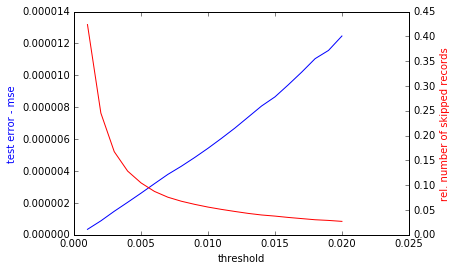
\includegraphics[width=2.5in]{img/error_impossible_threshold.png}
\caption{Error by threshold}
\label{fig_threshold}
\end{figure}

It turns out that the model for the authorized user also works very well for unauthorized users. So there is no profound difference in the mean squared error. But if we set the threshold to be very small (t = 0.001), the difference is greater. The impact on the authorized data can be seen in table \ref{table_model_quality}. Smoothing the error by a threshold reduces the variance and therefore makes the test error and the validation error more alike.

\subsection{Classification window}
To find the right window for classifying whether a user is authorized or not, we run some experiments. Figure \ref{fig_window} shows the smoothed mean squared error by window size and the resulting classification for a sequence of an authorized user. Moreover the blue line shows the number of records which were classified as predictable. The straight red line is the decision boundary. When the error is greater than this threshold the sequence is classified as unauthorized. The first 100 records are used as features. This means classification can start after 3 seconds. The figure shows that the chart converges to the right classification after about 190 time steps. We have to add the time steps of building the features. In total, we need in this case 290 time steps to classify correctly. This corresponds to 9.7 seconds. Also other examples show similar characteristics. Therefore 10 seconds seems to be a good estimate for a prototype. We will have to research in more detail whether we can reduce the window size because the longer the window the longer the potential unauthorized user can use the system.

\begin{figure}[!t]
\centering
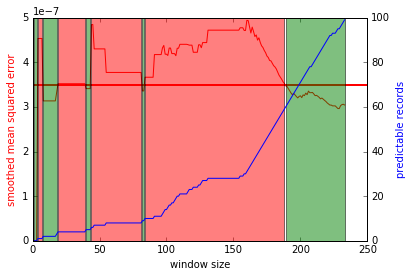
\includegraphics[width=2.5in]{img/window_size1.png}
\caption{Error by window size on authorized sequence}
\label{fig_window}
\end{figure}

\subsection{Evaluation}
To decide whether a data sequence is authorized or not, we need a decision boundary. We choose it by the lowest mean squared error which is seen for unauthorized users. We recorded 4 users for 10 seconds. This data serves as the unauthorized data. Using this approach we achieve a false accept rate (FAR) of 0\%, but a very high false reject rate (FRR) of 20\% on the test set. It turns out that the distance normed error is not suitable to compare the sequences because it doesn't seem to correlate with being authorized as well as the mean squared error based on time.

\section{Conclusion and future work}
\label{sec:conclusion}
We presented a mostly unsupervised approach to identify users by only training on the data of authorized user's mouse dynamics. The results show that mouse dynamics
contain a good amount of information, but it does not yet suffice for practical applications. The false reject rate of 20\% is too high. Since most of the other publications also included mouse events (i.e. \cite{zheng2011efficient}, \cite{pusara2004user}) into their model. Our results cannot be compared directly.

Future work has to focus on adding more features like mouse and keyboard events and how to incorporate them into the overall pipeline. This means we have to find a way to merge continuous cursor data with discrete events. The model should be also able to handle non-equidistant data points. 

Moreover we have to gather more user data to find a better estimate how to configure the threshold for impossible records and to set up the right decision boundary. Another way to improve the current method is to find an algorithm which better fits the mouse dynamics. One promising candidate could be Long Short-Term Memory (LSTM) Recurrent Neural Networks \cite{NIPS2014_5346}.

The source code for this project can be found on Github: \url{https://github.com/FelixNeutatz/BehavioralAuthentication} 

\section*{Acknowledgment}
Thank you, to all my fellow students who helped me to gather the data on which this work is based. Moreover I like to thank Professor Zhang Aixin for making it possible to put so much time and effort in this interesting topic.

% needed in second column of first page if using \IEEEpubid
%\IEEEpubidadjcol

% An example of a floating figure using the graphicx package.
% Note that \label must occur AFTER (or within) \caption.
% For figures, \caption should occur after the \includegraphics.
% Note that IEEEtran v1.7 and later has special internal code that
% is designed to preserve the operation of \label within \caption
% even when the captionsoff option is in effect. However, because
% of issues like this, it may be the safest practice to put all your
% \label just after \caption rather than within \caption{}.
%
% Reminder: the "draftcls" or "draftclsnofoot", not "draft", class
% option should be used if it is desired that the figures are to be
% displayed while in draft mode.
%
%\begin{figure}[!t]
%\centering
%\includegraphics[width=2.5in]{myfigure}
% where an .eps filename suffix will be assumed under latex, 
% and a .pdf suffix will be assumed for pdflatex; or what has been declared
% via \DeclareGraphicsExtensions.
%\caption{Simulation Results}
%\label{fig_sim}
%\end{figure}

% Note that IEEE typically puts floats only at the top, even when this
% results in a large percentage of a column being occupied by floats.


% An example of a double column floating figure using two subfigures.
% (The subfig.sty package must be loaded for this to work.)
% The subfigure \label commands are set within each subfloat command, the
% \label for the overall figure must come after \caption.
% \hfil must be used as a separator to get equal spacing.
% The subfigure.sty package works much the same way, except \subfigure is
% used instead of \subfloat.
%
%\begin{figure*}[!t]
%\centerline{\subfloat[Case I]\includegraphics[width=2.5in]{subfigcase1}%
%\label{fig_first_case}}
%\hfil
%\subfloat[Case II]{\includegraphics[width=2.5in]{subfigcase2}%
%\label{fig_second_case}}}
%\caption{Simulation results}
%\label{fig_sim}
%\end{figure*}
%
% Note that often IEEE papers with subfigures do not employ subfigure
% captions (using the optional argument to \subfloat), but instead will
% reference/describe all of them (a), (b), etc., within the main caption.


% An example of a floating table. Note that, for IEEE style tables, the 
% \caption command should come BEFORE the table. Table text will default to
% \footnotesize as IEEE normally uses this smaller font for tables.
% The \label must come after \caption as always.
%
%\begin{table}[!t]
%% increase table row spacing, adjust to taste
%\renewcommand{\arraystretch}{1.3}
% if using array.sty, it might be a good idea to tweak the value of
% \extrarowheight as needed to properly center the text within the cells
%\caption{An Example of a Table}
%\label{table_example}
%\centering
%% Some packages, such as MDW tools, offer better commands for making tables
%% than the plain LaTeX2e tabular which is used here.
%\begin{tabular}{|c||c|}
%\hline
%One & Two\\
%\hline
%Three & Four\\
%\hline
%\end{tabular}
%\end{table}


% Note that IEEE does not put floats in the very first column - or typically
% anywhere on the first page for that matter. Also, in-text middle ("here")
% positioning is not used. Most IEEE journals use top floats exclusively.
% Note that, LaTeX2e, unlike IEEE journals, places footnotes above bottom
% floats. This can be corrected via the \fnbelowfloat command of the
% stfloats package.









% if have a single appendix:
%\appendix[Proof of the Zonklar Equations]
% or
%\appendix  % for no appendix heading
% do not use \section anymore after \appendix, only \section*
% is possibly needed

% use appendices with more than one appendix
% then use \section to start each appendix
% you must declare a \section before using any
% \subsection or using \label (\appendices by itself
% starts a section numbered zero.)
%


%\appendices
%\section{Proof of the First Zonklar Equation}
%\blindtext

% use section* for acknowledgement
%\section*{Acknowledgment}
%The authors would like to thank...


% Can use something like this to put references on a page
% by themselves when using endfloat and the captionsoff option.
\ifCLASSOPTIONcaptionsoff
  \newpage
\fi



% trigger a \newpage just before the given reference
% number - used to balance the columns on the last page
% adjust value as needed - may need to be readjusted if
% the document is modified later
%\IEEEtriggeratref{8}
% The "triggered" command can be changed if desired:
%\IEEEtriggercmd{\enlargethispage{-5in}}

% references section

% can use a bibliography generated by BibTeX as a .bbl file
% BibTeX documentation can be easily obtained at:
% http://www.ctan.org/tex-archive/biblio/bibtex/contrib/doc/
% The IEEEtran BibTeX style support page is at:
% http://www.michaelshell.org/tex/ieeetran/bibtex/
%\bibliographystyle{IEEEtran}
% argument is your BibTeX string definitions and bibliography database(s)
%\bibliography{IEEEabrv,../bib/paper}
%
% <OR> manually copy in the resultant .bbl file
% set second argument of \begin to the number of references
% (used to reserve space for the reference number labels box)


\bibliographystyle{IEEEtran}
\bibliography{IEEEabrv,papers}


% biography section
% 
% If you have an EPS/PDF photo (graphicx package needed) extra braces are
% needed around the contents of the optional argument to biography to prevent
% the LaTeX parser from getting confused when it sees the complicated
% \includegraphics command within an optional argument. (You could create
% your own custom macro containing the \includegraphics command to make things
% simpler here.)
%\begin{biography}[{\includegraphics[width=1in,height=1.25in,clip,keepaspectratio]{mshell}}]{Michael Shell}
% or if you just want to reserve a space for a photo:

\begin{IEEEbiography}[{\includegraphics[width=1in,height=1.25in,clip,keepaspectratio]{picture}}]{John Doe}
\blindtext
\end{IEEEbiography}

% You can push biographies down or up by placing
% a \vfill before or after them. The appropriate
% use of \vfill depends on what kind of text is
% on the last page and whether or not the columns
% are being equalized.

%\vfill

% Can be used to pull up biographies so that the bottom of the last one
% is flush with the other column.
%\enlargethispage{-5in}




% that's all folks
\end{document}


